\documentclass{listhesis}
% --- Listhesis builds on KOMA script report (scrreprt).
%     Class arguments are passed to that class.

% --- Add additional packages here using \usepackage{package-name}.

% --- Provide your thesis details here.
\setup{%
  % de,                   % uncomment if your thesis is in German
  author=Iffat Brekhna, % your name
  title={Simulator Support for Dynamic Data Migration},
  date={May 31, 2018}, % submission date (today is used if unset)
  type=master,        % thesis type [master, bachelor, research, internship, diplom]
  advisor=Sven Rheindt M.Sc, % your advisor (typically some PhD. student)
  supervisor=Prof. Dr. sc. techn. Andreas Herkersdorf, % your supervisor
  % % uncomment the next lines if your thesis was carried out in industry
  % company=External Company,
  % externalAdvisor=Your Companyadvisor
}

\begin{document}

\maketitle
\cleardoublepage

% --- Thesis abstract.
%     For German thesis also provide an English version via the optional
%     argument: \anstract[English]{German}
\abstract{An abstract is defined as an abbreviated accurate
  representation of the contents of a document. -- American National
  Standards Institute (ANSI)}
\makeabstract
\clearpage

% --- Content tables.
\tableofcontents
\clearpage
\listoffigures
\clearpage
\listoftables
\clearpage

% --- Your thesis starts here.
%     Use \chapter{}, \section{}, \subsection{}, \subsubsection{},
%     and \paragraph{} to structure your thesis.

\chapter{Introduction}
This chapter serves as an introduction to the thesis. It explains the motivation for undertaking this work and the approach and concepts used in building the simulator support for dynamic data migration. Finally, the outline of the work is presented.
\section{Motivation}
Current research in semi-conductor industry is towards developing a single chip multi-tile multi-core processor. Hence, parallel programming is experiencing a rapid growth with the advent of architectures like the Invasic architecture as shown in Figure \ref{fig:multi-core,tile}. Because of multiple tiles and cores on one chip these processors deal with data processing at a high scale and complexity. Therefore, the bottleneck have shifted from computational complexities to data management capacities.\\
\\
Since modern, scalable multiprocessor system-on-chip (MPSoC) platforms have Non-Uniform Memory Access (NUMA) properties, application performance is highly influenced by data-to-task locality. The goal is to bring tasks and data closer together to increase overall performance. This is a twofold and complementary problem consisting of data and or task migration. In this thesis, we will look into data placement and see how it improves the performance of the MPSoC.\\
\newline
Figure \ref{fig:multi-core,tile} show a multi-tile multi-core processor architecture. Each tile has four Central Processing Units (CPU's) and a Tile Local Memory (TLM) which can be accessed by other tiles CPU's. Hence, there are local and remote accesses to the TLM. We need dynamic data placement in order to reduce these remote accesses at run time so that the distance of data from the core requesting the data is localized(minimized). Previously data was placed on the TLM's statically at compile time. However, this is not a very efficient or realistic way since in real life we don't know how an application or program will behave in the future. A more realistic way would be to dynamically place the data by examining the behavior of the processor for a given time interval and taking data placement decisions on that basis.
\begin{figure}
  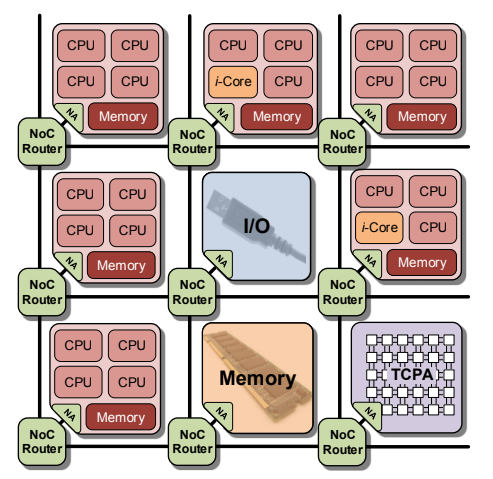
\includegraphics[width=0.5\linewidth]{multi-core,tile.png}
  \centering
  \caption{Invasic Architecture~\cite{iNetworkAdapter}}
  \label{fig:multi-core,tile}
\end{figure}
\section{Overview}
Figure \ref{fig:overviewOfSolution} shows the overview of the modules involved in dynamic migration scheme. Every cache module is connected to a cache{\_}stats module. All these cache{\_}stats modules and the TLM{\_}MEM modules report to the central TLM Stats module at every given time interval (T$_{interval}$). The central TLM Stats module does evaluation of this data and triggers migration if needed. \\
\\
Also, there is a vector address table which sits between the trace file and the CPU's as shown in Figure \ref{fig:traceFile}. This table contains the address translation of all the addresses from the DRAM to the TLM. At start all TLM's are empty which means every instruction has to access data from the DRAM. The vector address table is updated if the DRAM is accessed or if migration is triggered by the central TLM Stats module and that migration takes place.
\begin{figure}[h!]
  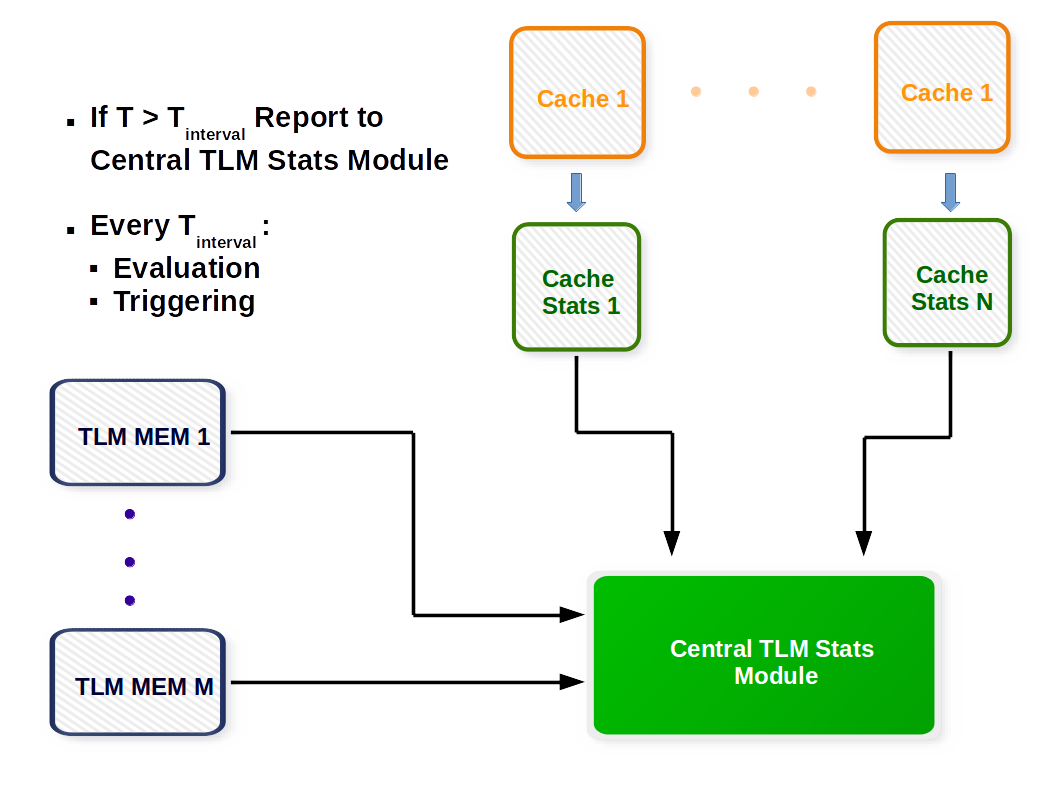
\includegraphics[width=0.7\linewidth]{overviewOfSolution.png}
  \centering
  \caption{Diagram showing overview of the modules used}
  \label{fig:overviewOfSolution}
\end{figure}
\begin{figure}[h!]
  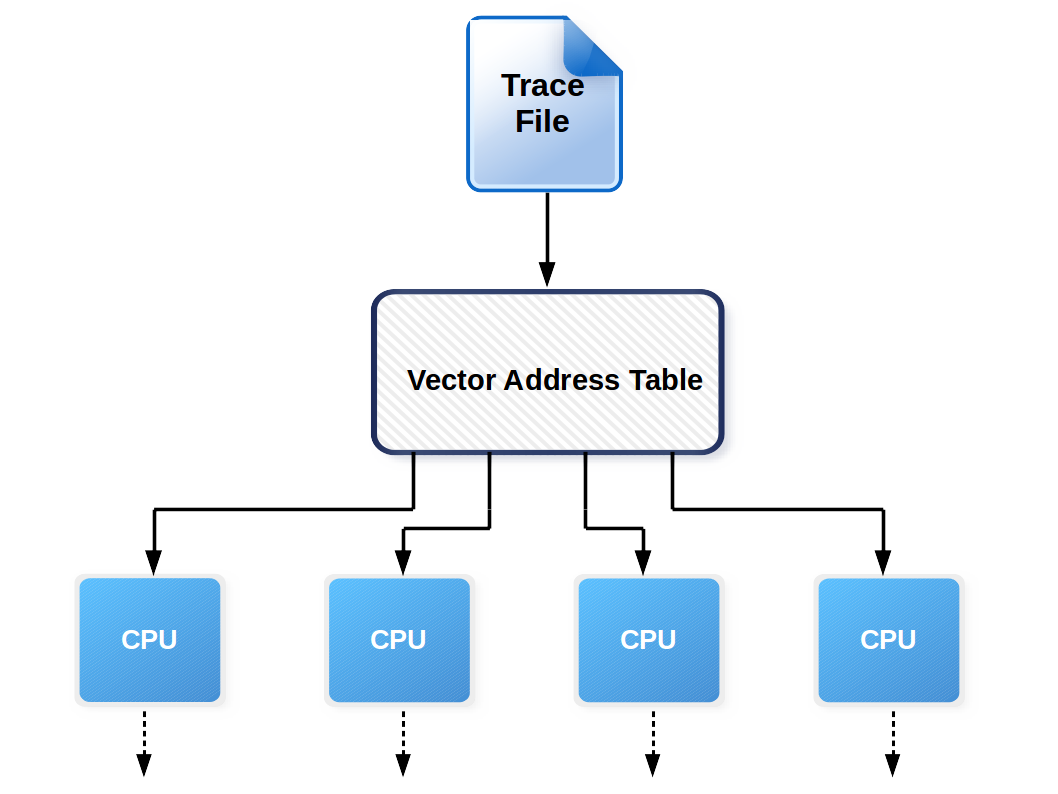
\includegraphics[width=0.7\linewidth]{traceFile.png}
  \centering
  \caption{Diagram showing where the trace file is placed}
  \label{fig:traceFile}
\end{figure}
\section{Outline}
The work is structured as follows. In Chapter 1, a brief introduction of the problem is given along with the motivation to solve it and then a brief overview of the solution is given.\\
\\
In Chapter 2, the overview of the existing system along with the current functionalities is given.\\
\\
In Chapter 3, the solution/approach is explained in detail and it is shown how the solution has been implemented. \\
\\
In Chapter 4, the results are presented. It shows how the performance has changed with the proposed solution implementation. \\
\\
In Chapter 5 a summary is given and some suggestions for future works in this domain. 
\chapter{Related Work/Background}
In this chapter the necessary background information is introduced in order to understand the thesis. The architecture is explained first followed by how data migration is handled in state-of-the art.\\
\\
\section{Main components explained}
\begin{figure}
  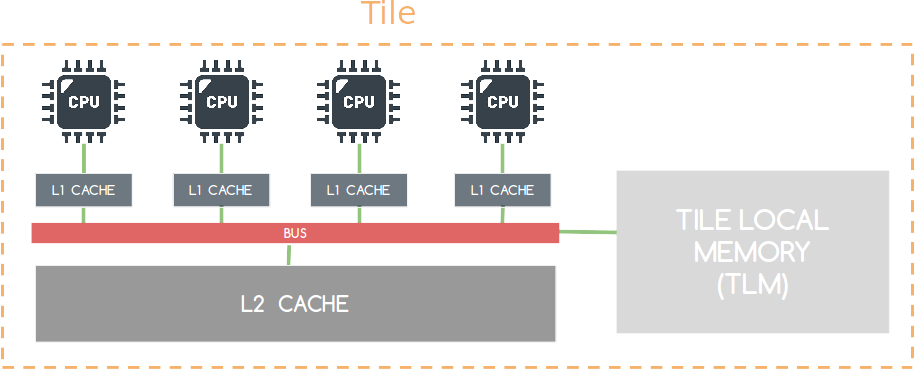
\includegraphics[width=\linewidth]{tile.png}
  \centering
  \caption{A tile}
  \label{fig:tile}
\end{figure}
\subsection{TLM}
TLM stands for Tile Local Memory. Each tile has its own TLM which is shared among all the processors of the tile~\cite{ankitThesis}. This memory is cachable by the L1 cache of the tile it sits on and by the L2 cache of any remote tile. The TLM from one tile can be accessed by the processor of another tile.\\
\subsection{Cache}
lskjdlsa
\subsection{Cache{\_}Stats Module}
The cache{\_}Stats module is connected to the L1 and L2 Cache modules and is continuously getting updates from them regarding cache hits, misses, evictions etc per cache line. This module bring all the data together and at the end of the simulation prints the compulsory misses,conflict misses, evictions, local misses, remote misses, local hits, remote hits for all the caches. This module also calculates the number of local and remote access to the TLM block by using all the metrics mentioned above.
\subsection{TLM{\_}MEM Module}
The TLM{\_}MEM module ??
\section{Data Placement/Migration for Caches}
Alot of work have been done on data-placement in the shared last level cache in order to reduce the distance of data from the core requesting the data and to take care of load balancing across the chip.\\
\\
In static data placement~\cite{cacheDataPlacement1},~\cite{cacheDataPlacement2} the whole address space is divided into subsets and every subset is mapped to a LLC slice regardless of the location of the requesting core which leads to unnecessary on-chip traffic. It’s advantage is that it evenly distributes the data among the available LLC slices and reduces off-chip accesses. In dynamic data placement~\cite{cacheDataPlacement1},~\cite{cacheDataPlacement3},~\cite{cacheDataPlacement4} the data blocks are placed such as to reduce the distance between the data block’s home node and the core requesting it. This eliminates the unnecessary on-chip traffic. It requires a lookup mechanism to locate the dynamically selected home node for each data block. In reactive data placement data is classified as private or shared using the operating systems page tables at page granularity~\cite{cacheDataPlacement4},~\cite{cacheDataPlacement6}. Because all placement is performed at page granularity level there is load imbalance as some LLC slices might have higher accesses compared to others. This load imbalance leads to hotspots~\cite{cacheDataPlacement6}.\\
\\
There is a hybrid data placement~\cite{cacheDataPlacement6} which combines the best features of static and dynamic data placement techniques. It optimizes data locality and also takes care of load balancing of the shared data. Hybrid data placement differs from Reactive data placement in regard to allocation of shared data among the cores i.e in Hybrid data placement, data is also classified as private or shared using the operating systems page tables but when a page is classified as shared (in hybrid data placement) it is allocated to a cluster of LLC slices and within this cluster the page is statically interleaved at the granularity of cache lines~\cite{cacheDataPlacement6}. This balances the load among the LLC slices.\\
\section{Task/Thread Placement}
Placing threads that share data on the same core improves performance~\cite{threadPlacement1}. However, finding the optimal mapping between threads and cores is a NP-hard problem~\cite{threadPlacement2} and cannot be scaled. One way to solve this problem is by monitoring the data accesses to determine the interaction between threads and the demands on cache memory~\cite{threadPlacement3}. In~\cite{threadPlacement3} a mechanism is there to transform the number of memory accesses from different threads to communication patterns and used these patterns to place the threads that share data on cores that share levels of cache.  They generate a communication matrix using the number of accesses to the same memory location by two threads and then maps the threads with highest communication to the same core. The disadvantage of this method is that generating the communication matrix through simulation is slow and they propose the application vendor provides this matrix with the application.\\
\\
In~\cite{threadPlacement4} a thread scheduling mechanism is proposed which uses the performance monitoring unit (PMU) with integrated hardware performance counters (HPCs) available in today’s processors to automatically re-cluster threads online. Using HPSs they monitor the stall breakdowns to check if cross chip communication is the reason for the stalls. If that is so, they detect the sharing pattern between the threads using the data sampling feature of the PMU.  For every thread they maintain a summary vector called the shMap  which holds the signature of data regions accessed by the thread which resulted in cross-chip communication. These shMaps are analyzed i.e threads with high degree of sharing will have similar shMaps and will be placed to the same cluster. The OS then migrates the threads with higher sharing to the same cluster and place them as close as possible~\cite{threadPlacement4}.\\
\section{Data+Thread Migration}
In~\cite{datathreadPlacement} a mechanism called CDCS is presented which using a combination of hardware and software techniques jointly places threads and data in multi-cores with distributed shared caches. CDCS takes a multi-step approach to solve the various interdependencies. It places data first and then places threads such that the threads are close to the center of mass of their data. Then using the thread placement it again re-place the data and once again for this data it re-places the threads to get a optimum placement. This technique improves performance and energy efficiency for both thread clustering and NUCA techniques~\cite{datathreadPlacement}.\\
\section{Dynamic Data Migration for TLM}
In~\cite{dynamicPageMigration} the authors have proposed a dynamic page migration scheme for a multiprocessor architecture using point-to-point interconnects with a distributed global memory. They use the \textit{pivot} mechanism to regulate the dynamic migration of pages by keeping track of the access pattern to every local page in every distributed memory module. If the access pattern is unbalanced then the page pivots to the nearest neighbor in the direction which caused the unbalanced access pattern.  

\chapter{Approach}
\section{Concept}
Fig. \ref{fig:approachOfSolution} shows the concept of the dynamic migration scheme. It shows what messages/data are exchanged between the different modules explained/introduced above. At every given time interval (T$_{interval}$) the cache{\_}stats module sends the number of local and remote accesses of a TLM block to the  central TLM Stats module and the TLM{\_}MEM module sends its free address space to the central TLM stats module. This block size is equal to a number of cache lines and can be varied. The central TLM Stats module evaluates this data and sends a migrate command to the L2 Cache{\_}stats module if migration shall be done.\\
\begin{figure}
  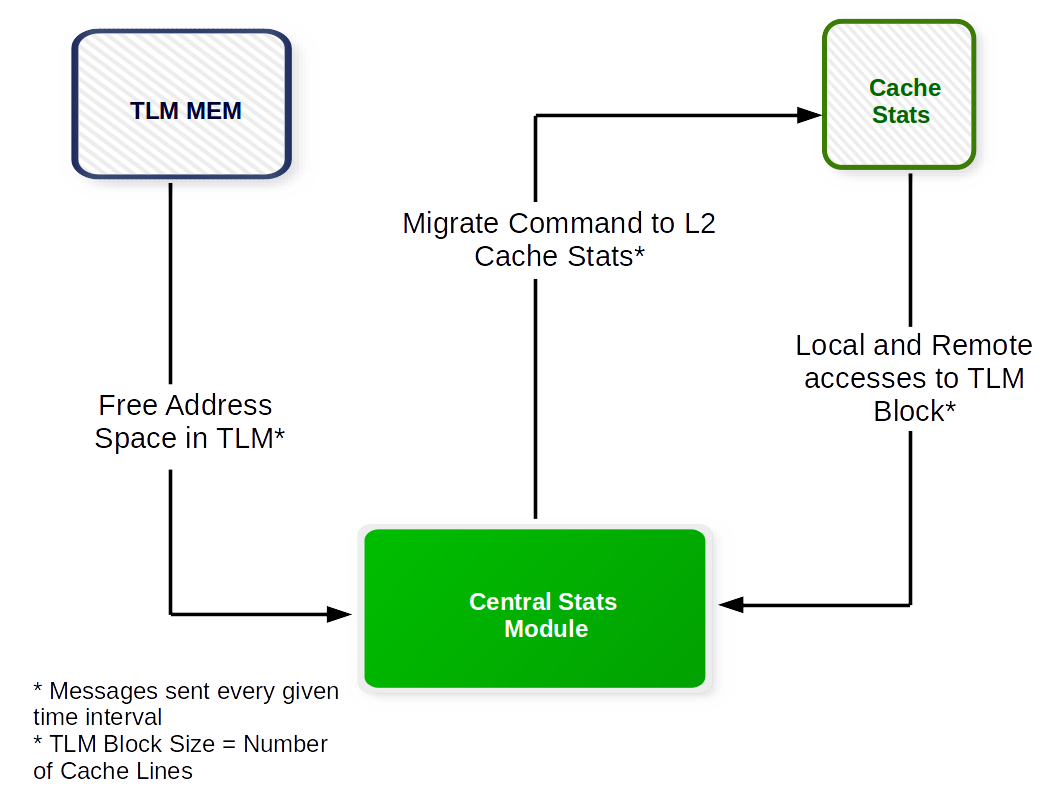
\includegraphics[width=0.7\linewidth]{approachOfSolution.png}
  \centering
  \caption{Diagram showing approach of the solution}
  \label{fig:approachOfSolution}
\end{figure}
\\
Fig. \ref{fig:remoteLocalAccess} shows the how the metric for local access and remote access is calculated in the cache{\_}stats module. The TLM which is being accessed is compared with the current tile. If the two values are equal it means it is a request to the TLM of the same tile which means its a local access. If the two values are different it means it is a request for another tile's TLM and it is checked whether there is a L1 cache hit. If there is a L1 cache hit it means it is a local access and if it is a miss it is checked whether it is a L2 cache hit. If it is a hit it means it is a local access and if it is a miss it means it is a remote access.\\
\begin{figure}
  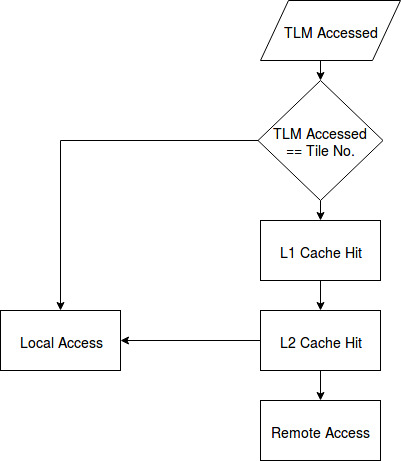
\includegraphics[width=0.5\linewidth]{remoteLocalAccess.jpg}
  \centering
  \caption{Flowchart showing process inside cache{\_}stats module}
  \label{fig:remoteLocalAccess}
\end{figure}
\\
Figure \ref{fig:freeSpaceTLM} shows how the free address space is calculated in the TLM{\_}MEM module. The vector address table is checked first and if it is empty it means all TLM's are empty. If the table is not empty and there is free space in a TLM, the starting and ending address of free space is extracted. If there is so free space in a TLM that is sent to the central TLM{\_}Stats module. \\
\begin{figure}
  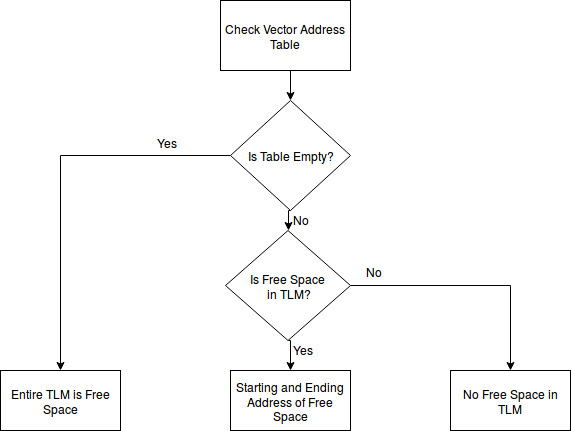
\includegraphics[width=0.7\linewidth]{freeSpaceTLM.jpg}
  \centering
  \caption{Flowchart showing how the free address space in TLM is calculated}
  \label{fig:freeSpaceTLM}
\end{figure}
\\
Figure \ref{fig:tlm_stats flowchart} shows the algorithm for determining when migration shall take place and which TLM block to migrate. First it is determined which node to migrate the TLM block to. This decision is based on the local and remote accesses to the specific TLM block. The tile with the maximum remote accesses to the TLM block is found and if these remote accesses are greater than local accesses to that TLM block it means it has to be migrated to the tile with the highest remote accesses. Then it is determined whether there is free space in the TLM of the tile to which the TLM block is to be migrated. If there is free space, a migration command is send to L2 Cache{\_|}Stats module. The migrate command is split to two commands, first reading data from the location from where data has to be migrated and then writing data at the new location. Once, the data is read a invalidation command is sent for that TLM Block/Cache Line(s) and the vector address table is updated. However, if there is no free space the block with the least number of local accesses is found in the TLM and that metric is compared with the remote accesses of the TLM block to be migrated. If the remote accesses metric is higher than the local accesses of the block with least number of local accesses a migration command is send to the L2 Cache{\_|}Stats module for this block i.e this block is migrated back to the DDR and free space is made for the incoming TLM block. Now with free space in the TLM a migration command is send to the  L2 Cache{\_|}Stats module for the block to be migrated.\\
\\
\begin{figure}
  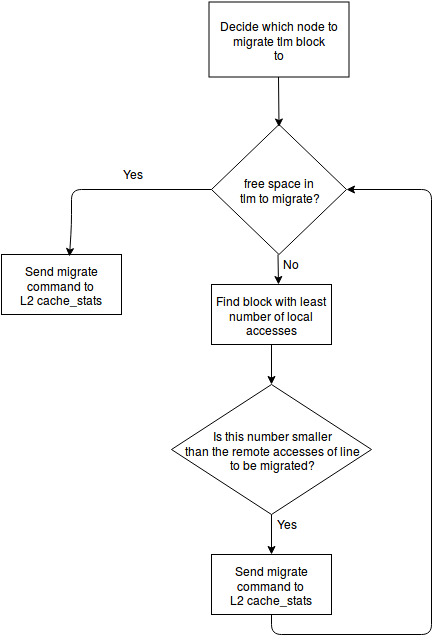
\includegraphics[width=0.7\linewidth]{tlm_stats(1).jpg}
  \centering
  \caption{Flowchart showing process inside central TLM{\_}STATS module}
  \label{fig:tlm_stats flowchart}
\end{figure}

\chapter{Evaluation}

\chapter{Conclusion and Outlook}


% --- Bibliography
\cleardoublepage
\bibliographystyle{plain}
\bibliography{thesis}

% --- Mandatory confirmation.
\confirmation

\end{document}

%%% Local Variables:
%%% mode: latex
%%% TeX-master: t
%%% End:
